\documentclass[twoside]{book}

% Packages required by doxygen
\usepackage{fixltx2e}
\usepackage{calc}
\usepackage{doxygen}
\usepackage[export]{adjustbox} % also loads graphicx
\usepackage{graphicx}
\usepackage[utf8]{inputenc}
\usepackage{makeidx}
\usepackage{multicol}
\usepackage{multirow}
\PassOptionsToPackage{warn}{textcomp}
\usepackage{textcomp}
\usepackage[nointegrals]{wasysym}
\usepackage[table]{xcolor}

% Font selection
\usepackage[T1]{fontenc}
\usepackage[scaled=.90]{helvet}
\usepackage{courier}
\usepackage{amssymb}
\usepackage{sectsty}
\renewcommand{\familydefault}{\sfdefault}
\allsectionsfont{%
  \fontseries{bc}\selectfont%
  \color{darkgray}%
}
\renewcommand{\DoxyLabelFont}{%
  \fontseries{bc}\selectfont%
  \color{darkgray}%
}
\newcommand{\+}{\discretionary{\mbox{\scriptsize$\hookleftarrow$}}{}{}}

% Page & text layout
\usepackage{geometry}
\geometry{%
  a4paper,%
  top=2.5cm,%
  bottom=2.5cm,%
  left=2.5cm,%
  right=2.5cm%
}
\tolerance=750
\hfuzz=15pt
\hbadness=750
\setlength{\emergencystretch}{15pt}
\setlength{\parindent}{0cm}
\setlength{\parskip}{3ex plus 2ex minus 2ex}
\makeatletter
\renewcommand{\paragraph}{%
  \@startsection{paragraph}{4}{0ex}{-1.0ex}{1.0ex}{%
    \normalfont\normalsize\bfseries\SS@parafont%
  }%
}
\renewcommand{\subparagraph}{%
  \@startsection{subparagraph}{5}{0ex}{-1.0ex}{1.0ex}{%
    \normalfont\normalsize\bfseries\SS@subparafont%
  }%
}
\makeatother

% Headers & footers
\usepackage{fancyhdr}
\pagestyle{fancyplain}
\fancyhead[LE]{\fancyplain{}{\bfseries\thepage}}
\fancyhead[CE]{\fancyplain{}{}}
\fancyhead[RE]{\fancyplain{}{\bfseries\leftmark}}
\fancyhead[LO]{\fancyplain{}{\bfseries\rightmark}}
\fancyhead[CO]{\fancyplain{}{}}
\fancyhead[RO]{\fancyplain{}{\bfseries\thepage}}
\fancyfoot[LE]{\fancyplain{}{}}
\fancyfoot[CE]{\fancyplain{}{}}
\fancyfoot[RE]{\fancyplain{}{\bfseries\scriptsize Generated by Doxygen }}
\fancyfoot[LO]{\fancyplain{}{\bfseries\scriptsize Generated by Doxygen }}
\fancyfoot[CO]{\fancyplain{}{}}
\fancyfoot[RO]{\fancyplain{}{}}
\renewcommand{\footrulewidth}{0.4pt}
\renewcommand{\chaptermark}[1]{%
  \markboth{#1}{}%
}
\renewcommand{\sectionmark}[1]{%
  \markright{\thesection\ #1}%
}

% Indices & bibliography
\usepackage{natbib}
\usepackage[titles]{tocloft}
\setcounter{tocdepth}{3}
\setcounter{secnumdepth}{5}
\makeindex

% Hyperlinks (required, but should be loaded last)
\usepackage{ifpdf}
\ifpdf
  \usepackage[pdftex,pagebackref=true]{hyperref}
\else
  \usepackage[ps2pdf,pagebackref=true]{hyperref}
\fi
\hypersetup{%
  colorlinks=true,%
  linkcolor=blue,%
  citecolor=blue,%
  unicode%
}

% Custom commands
\newcommand{\clearemptydoublepage}{%
  \newpage{\pagestyle{empty}\cleardoublepage}%
}

\usepackage{caption}
\captionsetup{labelsep=space,justification=centering,font={bf},singlelinecheck=off,skip=4pt,position=top}

%===== C O N T E N T S =====

\begin{document}

% Titlepage & ToC
\hypersetup{pageanchor=false,
             bookmarksnumbered=true,
             pdfencoding=unicode
            }
\pagenumbering{roman}
\begin{titlepage}
\vspace*{7cm}
\begin{center}%
{\Large My Project }\\
\vspace*{1cm}
{\large Generated by Doxygen 1.8.11}\\
\end{center}
\end{titlepage}
\clearemptydoublepage
\tableofcontents
\clearemptydoublepage
\pagenumbering{arabic}
\hypersetup{pageanchor=true}

%--- Begin generated contents ---
\chapter{Hierarchical Index}
\section{Class Hierarchy}
This inheritance list is sorted roughly, but not completely, alphabetically\+:\begin{DoxyCompactList}
\item \contentsline{section}{Figura}{\pageref{classFigura}}{}
\begin{DoxyCompactList}
\item \contentsline{section}{Circulo}{\pageref{classCirculo}}{}
\item \contentsline{section}{Cuadrado}{\pageref{classCuadrado}}{}
\item \contentsline{section}{Triangulo}{\pageref{classTriangulo}}{}
\end{DoxyCompactList}
\end{DoxyCompactList}

\chapter{Class Index}
\section{Class List}
Here are the classes, structs, unions and interfaces with brief descriptions\+:\begin{DoxyCompactList}
\item\contentsline{section}{\hyperlink{classCirculo}{Circulo} }{\pageref{classCirculo}}{}
\item\contentsline{section}{\hyperlink{classCuadrado}{Cuadrado} }{\pageref{classCuadrado}}{}
\item\contentsline{section}{\hyperlink{classFigura}{Figura} }{\pageref{classFigura}}{}
\item\contentsline{section}{\hyperlink{classTriangulo}{Triangulo} }{\pageref{classTriangulo}}{}
\end{DoxyCompactList}

\chapter{Class Documentation}
\hypertarget{classCirculo}{}\section{Circulo Class Reference}
\label{classCirculo}\index{Circulo@{Circulo}}


{\ttfamily \#include $<$circulo.\+h$>$}



Inheritance diagram for Circulo\+:
\nopagebreak
\begin{figure}[H]
\begin{center}
\leavevmode
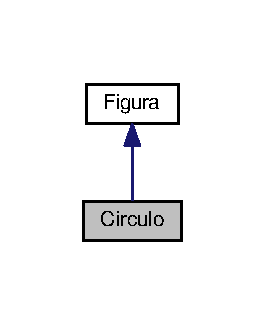
\includegraphics[width=127pt]{classCirculo__inherit__graph}
\end{center}
\end{figure}


Collaboration diagram for Circulo\+:
\nopagebreak
\begin{figure}[H]
\begin{center}
\leavevmode
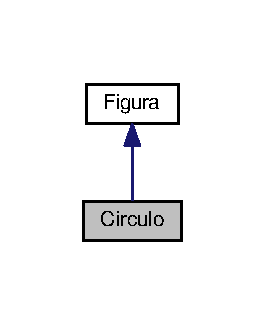
\includegraphics[width=127pt]{classCirculo__coll__graph}
\end{center}
\end{figure}
\subsection*{Public Member Functions}
\begin{DoxyCompactItemize}
\item 
\hyperlink{classCirculo_a6933bf908b78a4167684081a3a8f257f}{Circulo} ()
\item 
virtual \hyperlink{classCirculo_a8efe39e0e89487519cd802f0738d3bf4}{$\sim$\+Circulo} ()
\item 
virtual double \hyperlink{classCirculo_aded0c4ee374eb000f59d8d8da01ad72d}{area} ()
\item 
virtual double \hyperlink{classCirculo_acc35f8fdd7303fca9fe54b0da458bdf2}{perimetro} ()
\item 
void \hyperlink{classCirculo_a8db226b0c3bad5b8a01d60afb45838c7}{operator$\sim$} ()
\item 
void \hyperlink{classCirculo_a64bd2cabfdbca872d44bf1eb13f59cbb}{operator!} ()
\end{DoxyCompactItemize}
\subsection*{Additional Inherited Members}


\subsection{Detailed Description}
Clase que representa un círculo. 

\subsection{Constructor \& Destructor Documentation}
\index{Circulo@{Circulo}!Circulo@{Circulo}}
\index{Circulo@{Circulo}!Circulo@{Circulo}}
\subsubsection[{\texorpdfstring{Circulo()}{Circulo()}}]{\setlength{\rightskip}{0pt plus 5cm}Circulo\+::\+Circulo (
\begin{DoxyParamCaption}
{}
\end{DoxyParamCaption}
)}\hypertarget{classCirculo_a6933bf908b78a4167684081a3a8f257f}{}\label{classCirculo_a6933bf908b78a4167684081a3a8f257f}
Constructor por defecto. Crea un circulo de radio 1 \index{Circulo@{Circulo}!````~Circulo@{$\sim$\+Circulo}}
\index{````~Circulo@{$\sim$\+Circulo}!Circulo@{Circulo}}
\subsubsection[{\texorpdfstring{$\sim$\+Circulo()}{~Circulo()}}]{\setlength{\rightskip}{0pt plus 5cm}Circulo\+::$\sim$\+Circulo (
\begin{DoxyParamCaption}
{}
\end{DoxyParamCaption}
)\hspace{0.3cm}{\ttfamily [virtual]}}\hypertarget{classCirculo_a8efe39e0e89487519cd802f0738d3bf4}{}\label{classCirculo_a8efe39e0e89487519cd802f0738d3bf4}
Destructor por defecto. 

\subsection{Member Function Documentation}
\index{Circulo@{Circulo}!area@{area}}
\index{area@{area}!Circulo@{Circulo}}
\subsubsection[{\texorpdfstring{area()}{area()}}]{\setlength{\rightskip}{0pt plus 5cm}double Circulo\+::area (
\begin{DoxyParamCaption}
{}
\end{DoxyParamCaption}
)\hspace{0.3cm}{\ttfamily [virtual]}}\hypertarget{classCirculo_aded0c4ee374eb000f59d8d8da01ad72d}{}\label{classCirculo_aded0c4ee374eb000f59d8d8da01ad72d}
Calcula el área del cuadrado. \begin{DoxyReturn}{Returns}
El resultado del cálculo. 
\end{DoxyReturn}


Reimplemented from \hyperlink{classFigura_ade6b12995c86cb72e37738668d77963d}{Figura}.

\index{Circulo@{Circulo}!operator"!@{operator"!}}
\index{operator"!@{operator"!}!Circulo@{Circulo}}
\subsubsection[{\texorpdfstring{operator"!()}{operator!()}}]{\setlength{\rightskip}{0pt plus 5cm}void Circulo\+::operator! (
\begin{DoxyParamCaption}
{}
\end{DoxyParamCaption}
)}\hypertarget{classCirculo_a64bd2cabfdbca872d44bf1eb13f59cbb}{}\label{classCirculo_a64bd2cabfdbca872d44bf1eb13f59cbb}
Imprime el area y el perimetro. \index{Circulo@{Circulo}!operator````~@{operator$\sim$}}
\index{operator````~@{operator$\sim$}!Circulo@{Circulo}}
\subsubsection[{\texorpdfstring{operator$\sim$()}{operator~()}}]{\setlength{\rightskip}{0pt plus 5cm}void Circulo\+::operator$\sim$ (
\begin{DoxyParamCaption}
{}
\end{DoxyParamCaption}
)}\hypertarget{classCirculo_a8db226b0c3bad5b8a01d60afb45838c7}{}\label{classCirculo_a8db226b0c3bad5b8a01d60afb45838c7}
Imprime los datos del cuadrado. \index{Circulo@{Circulo}!perimetro@{perimetro}}
\index{perimetro@{perimetro}!Circulo@{Circulo}}
\subsubsection[{\texorpdfstring{perimetro()}{perimetro()}}]{\setlength{\rightskip}{0pt plus 5cm}double Circulo\+::perimetro (
\begin{DoxyParamCaption}
{}
\end{DoxyParamCaption}
)\hspace{0.3cm}{\ttfamily [virtual]}}\hypertarget{classCirculo_acc35f8fdd7303fca9fe54b0da458bdf2}{}\label{classCirculo_acc35f8fdd7303fca9fe54b0da458bdf2}
Calcula el perímetro del cuadrado \begin{DoxyReturn}{Returns}
El resultado del cálculo. 
\end{DoxyReturn}


Reimplemented from \hyperlink{classFigura_a7451dfc1da3533fa15205df11afe7ac3}{Figura}.



The documentation for this class was generated from the following files\+:\begin{DoxyCompactItemize}
\item 
include/circulo.\+h\item 
source/circulo.\+cpp\end{DoxyCompactItemize}

\hypertarget{classCuadrado}{}\section{Cuadrado Class Reference}
\label{classCuadrado}\index{Cuadrado@{Cuadrado}}


{\ttfamily \#include $<$cuadrado.\+h$>$}



Inheritance diagram for Cuadrado\+:
\nopagebreak
\begin{figure}[H]
\begin{center}
\leavevmode
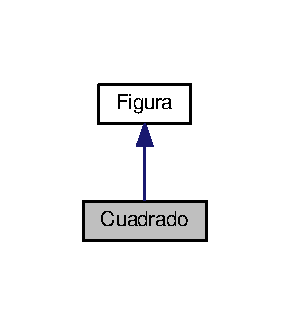
\includegraphics[width=139pt]{classCuadrado__inherit__graph}
\end{center}
\end{figure}


Collaboration diagram for Cuadrado\+:
\nopagebreak
\begin{figure}[H]
\begin{center}
\leavevmode
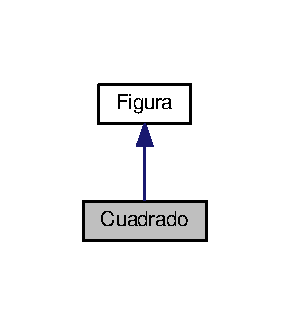
\includegraphics[width=139pt]{classCuadrado__coll__graph}
\end{center}
\end{figure}
\subsection*{Public Member Functions}
\begin{DoxyCompactItemize}
\item 
\hyperlink{classCuadrado_ad28d9dddc29e1987ec620b07b0a4acc9}{Cuadrado} ()
\item 
virtual \hyperlink{classCuadrado_a9f5bf29c9b8368ad45a4a3c12f9fd7c2}{$\sim$\+Cuadrado} ()
\item 
virtual double \hyperlink{classCuadrado_a379a755de0b95f295e30e6049e19426c}{area} ()
\item 
virtual double \hyperlink{classCuadrado_aa7072852e41bde681376b57503495c74}{perimetro} ()
\item 
void \hyperlink{classCuadrado_a6303f81de8d357f415d00a116b73a6fc}{operator$\sim$} ()
\item 
void \hyperlink{classCuadrado_a78be5dcef640ad7f82858f44fb623af5}{operator!} ()
\end{DoxyCompactItemize}
\subsection*{Additional Inherited Members}


\subsection{Detailed Description}
Clase que representa un cuadrado. 

\subsection{Constructor \& Destructor Documentation}
\index{Cuadrado@{Cuadrado}!Cuadrado@{Cuadrado}}
\index{Cuadrado@{Cuadrado}!Cuadrado@{Cuadrado}}
\subsubsection[{\texorpdfstring{Cuadrado()}{Cuadrado()}}]{\setlength{\rightskip}{0pt plus 5cm}Cuadrado\+::\+Cuadrado (
\begin{DoxyParamCaption}
{}
\end{DoxyParamCaption}
)}\hypertarget{classCuadrado_ad28d9dddc29e1987ec620b07b0a4acc9}{}\label{classCuadrado_ad28d9dddc29e1987ec620b07b0a4acc9}
Constructor por defecto. Crea un cuadrado de lado 3 \index{Cuadrado@{Cuadrado}!````~Cuadrado@{$\sim$\+Cuadrado}}
\index{````~Cuadrado@{$\sim$\+Cuadrado}!Cuadrado@{Cuadrado}}
\subsubsection[{\texorpdfstring{$\sim$\+Cuadrado()}{~Cuadrado()}}]{\setlength{\rightskip}{0pt plus 5cm}Cuadrado\+::$\sim$\+Cuadrado (
\begin{DoxyParamCaption}
{}
\end{DoxyParamCaption}
)\hspace{0.3cm}{\ttfamily [virtual]}}\hypertarget{classCuadrado_a9f5bf29c9b8368ad45a4a3c12f9fd7c2}{}\label{classCuadrado_a9f5bf29c9b8368ad45a4a3c12f9fd7c2}
Destructor por defecto. 

\subsection{Member Function Documentation}
\index{Cuadrado@{Cuadrado}!area@{area}}
\index{area@{area}!Cuadrado@{Cuadrado}}
\subsubsection[{\texorpdfstring{area()}{area()}}]{\setlength{\rightskip}{0pt plus 5cm}double Cuadrado\+::area (
\begin{DoxyParamCaption}
{}
\end{DoxyParamCaption}
)\hspace{0.3cm}{\ttfamily [virtual]}}\hypertarget{classCuadrado_a379a755de0b95f295e30e6049e19426c}{}\label{classCuadrado_a379a755de0b95f295e30e6049e19426c}
Calcula el área del cuadrado. \begin{DoxyReturn}{Returns}
El resultado del cálculo. 
\end{DoxyReturn}


Reimplemented from \hyperlink{classFigura_ade6b12995c86cb72e37738668d77963d}{Figura}.

\index{Cuadrado@{Cuadrado}!operator"!@{operator"!}}
\index{operator"!@{operator"!}!Cuadrado@{Cuadrado}}
\subsubsection[{\texorpdfstring{operator"!()}{operator!()}}]{\setlength{\rightskip}{0pt plus 5cm}void Cuadrado\+::operator! (
\begin{DoxyParamCaption}
{}
\end{DoxyParamCaption}
)}\hypertarget{classCuadrado_a78be5dcef640ad7f82858f44fb623af5}{}\label{classCuadrado_a78be5dcef640ad7f82858f44fb623af5}
Imprime el area y el perimetro. \index{Cuadrado@{Cuadrado}!operator````~@{operator$\sim$}}
\index{operator````~@{operator$\sim$}!Cuadrado@{Cuadrado}}
\subsubsection[{\texorpdfstring{operator$\sim$()}{operator~()}}]{\setlength{\rightskip}{0pt plus 5cm}void Cuadrado\+::operator$\sim$ (
\begin{DoxyParamCaption}
{}
\end{DoxyParamCaption}
)}\hypertarget{classCuadrado_a6303f81de8d357f415d00a116b73a6fc}{}\label{classCuadrado_a6303f81de8d357f415d00a116b73a6fc}
Imprime los datos del cuadrado. \index{Cuadrado@{Cuadrado}!perimetro@{perimetro}}
\index{perimetro@{perimetro}!Cuadrado@{Cuadrado}}
\subsubsection[{\texorpdfstring{perimetro()}{perimetro()}}]{\setlength{\rightskip}{0pt plus 5cm}double Cuadrado\+::perimetro (
\begin{DoxyParamCaption}
{}
\end{DoxyParamCaption}
)\hspace{0.3cm}{\ttfamily [virtual]}}\hypertarget{classCuadrado_aa7072852e41bde681376b57503495c74}{}\label{classCuadrado_aa7072852e41bde681376b57503495c74}
Calcula el perímetro del cuadrado \begin{DoxyReturn}{Returns}
El resultado del cálculo. 
\end{DoxyReturn}


Reimplemented from \hyperlink{classFigura_a7451dfc1da3533fa15205df11afe7ac3}{Figura}.



The documentation for this class was generated from the following files\+:\begin{DoxyCompactItemize}
\item 
include/cuadrado.\+h\item 
source/cuadrado.\+cpp\end{DoxyCompactItemize}

\hypertarget{classFigura}{}\section{Figura Class Reference}
\label{classFigura}\index{Figura@{Figura}}


{\ttfamily \#include $<$figura.\+h$>$}



Inheritance diagram for Figura\+:
\nopagebreak
\begin{figure}[H]
\begin{center}
\leavevmode
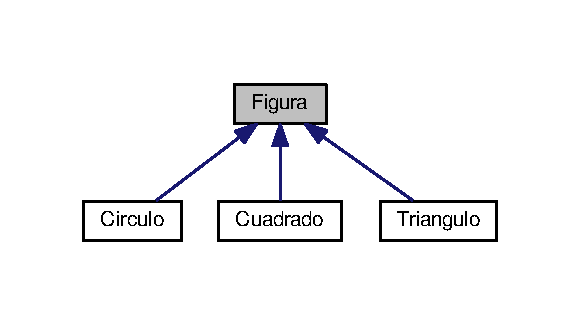
\includegraphics[width=279pt]{classFigura__inherit__graph}
\end{center}
\end{figure}
\subsection*{Public Member Functions}
\begin{DoxyCompactItemize}
\item 
{\bfseries Figura} (char $\ast$v\+\_\+nombre, char $\ast$v\+\_\+color)\hypertarget{classFigura_a11d2d8d29aee9f74b813df7abdbb4971}{}\label{classFigura_a11d2d8d29aee9f74b813df7abdbb4971}

\item 
virtual double \hyperlink{classFigura_ade6b12995c86cb72e37738668d77963d}{area} ()
\item 
virtual double \hyperlink{classFigura_a7451dfc1da3533fa15205df11afe7ac3}{perimetro} ()
\item 
void \hyperlink{classFigura_a1a66a42a0eed6dcacfb410d970780fa5}{set\+Nombre} (char $\ast$v\+\_\+nombre)
\item 
void \hyperlink{classFigura_ac593544158f072cf57835892cc35096e}{set\+Color} (char $\ast$v\+\_\+color)
\item 
std\+::string \hyperlink{classFigura_ad33b005e0206b70251e652f53796d586}{get\+Nombre} ()
\item 
std\+::string \hyperlink{classFigura_a940226fafa4e275b6a48dcff09fb5927}{get\+Color} ()
\end{DoxyCompactItemize}
\subsection*{Protected Attributes}
\begin{DoxyCompactItemize}
\item 
std\+::string \hyperlink{classFigura_a67df59705ff131e5a56fe4d4af3cfb73}{nombre}
\item 
std\+::string \hyperlink{classFigura_ab27a1a9f1236ad5ce14fce5776ed3aea}{color}
\end{DoxyCompactItemize}


\subsection{Detailed Description}
Clase que representa una figura. Define funciones básicas que debe tener cualquier otra clase derivada. 

\subsection{Member Function Documentation}
\index{Figura@{Figura}!area@{area}}
\index{area@{area}!Figura@{Figura}}
\subsubsection[{\texorpdfstring{area()}{area()}}]{\setlength{\rightskip}{0pt plus 5cm}double Figura\+::area (
\begin{DoxyParamCaption}
{}
\end{DoxyParamCaption}
)\hspace{0.3cm}{\ttfamily [virtual]}}\hypertarget{classFigura_ade6b12995c86cb72e37738668d77963d}{}\label{classFigura_ade6b12995c86cb72e37738668d77963d}
Función que calcula el área de la figura. Se puede reimplementar en clases derivadas. \begin{DoxyReturn}{Returns}
Para objetos \hyperlink{classFigura}{Figura} puros devuelve 0 siempre. 
\end{DoxyReturn}


Reimplemented in \hyperlink{classTriangulo_a1c71a04df8caa1bcb52898636fb20004}{Triangulo}, \hyperlink{classCirculo_aded0c4ee374eb000f59d8d8da01ad72d}{Circulo}, and \hyperlink{classCuadrado_a379a755de0b95f295e30e6049e19426c}{Cuadrado}.

\index{Figura@{Figura}!get\+Color@{get\+Color}}
\index{get\+Color@{get\+Color}!Figura@{Figura}}
\subsubsection[{\texorpdfstring{get\+Color()}{getColor()}}]{\setlength{\rightskip}{0pt plus 5cm}std\+::string Figura\+::get\+Color (
\begin{DoxyParamCaption}
{}
\end{DoxyParamCaption}
)}\hypertarget{classFigura_a940226fafa4e275b6a48dcff09fb5927}{}\label{classFigura_a940226fafa4e275b6a48dcff09fb5927}
Devuelve el color de la figura. \begin{DoxyReturn}{Returns}
El color. 
\end{DoxyReturn}
\index{Figura@{Figura}!get\+Nombre@{get\+Nombre}}
\index{get\+Nombre@{get\+Nombre}!Figura@{Figura}}
\subsubsection[{\texorpdfstring{get\+Nombre()}{getNombre()}}]{\setlength{\rightskip}{0pt plus 5cm}std\+::string Figura\+::get\+Nombre (
\begin{DoxyParamCaption}
{}
\end{DoxyParamCaption}
)}\hypertarget{classFigura_ad33b005e0206b70251e652f53796d586}{}\label{classFigura_ad33b005e0206b70251e652f53796d586}
Devuelve el nombre de la figura. \begin{DoxyReturn}{Returns}
El nombre. 
\end{DoxyReturn}
\index{Figura@{Figura}!perimetro@{perimetro}}
\index{perimetro@{perimetro}!Figura@{Figura}}
\subsubsection[{\texorpdfstring{perimetro()}{perimetro()}}]{\setlength{\rightskip}{0pt plus 5cm}double Figura\+::perimetro (
\begin{DoxyParamCaption}
{}
\end{DoxyParamCaption}
)\hspace{0.3cm}{\ttfamily [virtual]}}\hypertarget{classFigura_a7451dfc1da3533fa15205df11afe7ac3}{}\label{classFigura_a7451dfc1da3533fa15205df11afe7ac3}
Función que calcula el perímetro de la figura. Se puede reimplementar en clases derivadas. \begin{DoxyReturn}{Returns}
Para objetos \hyperlink{classFigura}{Figura} puros devuelve 0 siempre. 
\end{DoxyReturn}


Reimplemented in \hyperlink{classTriangulo_a6f5c542675a726b35f48f953bb2d9acf}{Triangulo}, \hyperlink{classCirculo_acc35f8fdd7303fca9fe54b0da458bdf2}{Circulo}, and \hyperlink{classCuadrado_aa7072852e41bde681376b57503495c74}{Cuadrado}.

\index{Figura@{Figura}!set\+Color@{set\+Color}}
\index{set\+Color@{set\+Color}!Figura@{Figura}}
\subsubsection[{\texorpdfstring{set\+Color(char $\ast$v\+\_\+color)}{setColor(char *v_color)}}]{\setlength{\rightskip}{0pt plus 5cm}void Figura\+::set\+Color (
\begin{DoxyParamCaption}
\item[{char $\ast$}]{v\+\_\+color}
\end{DoxyParamCaption}
)}\hypertarget{classFigura_ac593544158f072cf57835892cc35096e}{}\label{classFigura_ac593544158f072cf57835892cc35096e}
Cambia el color de la figura. 
\begin{DoxyParams}{Parameters}
{\em v\+\_\+color} & El nuevo color. \\
\hline
\end{DoxyParams}
\index{Figura@{Figura}!set\+Nombre@{set\+Nombre}}
\index{set\+Nombre@{set\+Nombre}!Figura@{Figura}}
\subsubsection[{\texorpdfstring{set\+Nombre(char $\ast$v\+\_\+nombre)}{setNombre(char *v_nombre)}}]{\setlength{\rightskip}{0pt plus 5cm}void Figura\+::set\+Nombre (
\begin{DoxyParamCaption}
\item[{char $\ast$}]{v\+\_\+nombre}
\end{DoxyParamCaption}
)}\hypertarget{classFigura_a1a66a42a0eed6dcacfb410d970780fa5}{}\label{classFigura_a1a66a42a0eed6dcacfb410d970780fa5}
Cambia el nombre de la figura. 
\begin{DoxyParams}{Parameters}
{\em v\+\_\+nombre} & El nuevo nombre. \\
\hline
\end{DoxyParams}


\subsection{Member Data Documentation}
\index{Figura@{Figura}!color@{color}}
\index{color@{color}!Figura@{Figura}}
\subsubsection[{\texorpdfstring{color}{color}}]{\setlength{\rightskip}{0pt plus 5cm}std\+::string Figura\+::color\hspace{0.3cm}{\ttfamily [protected]}}\hypertarget{classFigura_ab27a1a9f1236ad5ce14fce5776ed3aea}{}\label{classFigura_ab27a1a9f1236ad5ce14fce5776ed3aea}
Color de la figura. \index{Figura@{Figura}!nombre@{nombre}}
\index{nombre@{nombre}!Figura@{Figura}}
\subsubsection[{\texorpdfstring{nombre}{nombre}}]{\setlength{\rightskip}{0pt plus 5cm}std\+::string Figura\+::nombre\hspace{0.3cm}{\ttfamily [protected]}}\hypertarget{classFigura_a67df59705ff131e5a56fe4d4af3cfb73}{}\label{classFigura_a67df59705ff131e5a56fe4d4af3cfb73}
Nombre de la figura. 

The documentation for this class was generated from the following files\+:\begin{DoxyCompactItemize}
\item 
include/figura.\+h\item 
source/figura.\+cpp\end{DoxyCompactItemize}

\hypertarget{classTriangulo}{}\section{Triangulo Class Reference}
\label{classTriangulo}\index{Triangulo@{Triangulo}}


{\ttfamily \#include $<$triangulo.\+h$>$}



Inheritance diagram for Triangulo\+:
\nopagebreak
\begin{figure}[H]
\begin{center}
\leavevmode
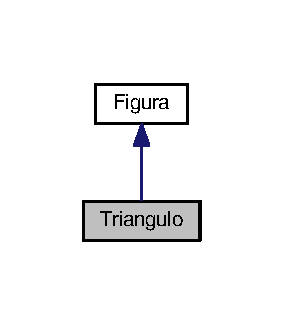
\includegraphics[width=136pt]{classTriangulo__inherit__graph}
\end{center}
\end{figure}


Collaboration diagram for Triangulo\+:
\nopagebreak
\begin{figure}[H]
\begin{center}
\leavevmode
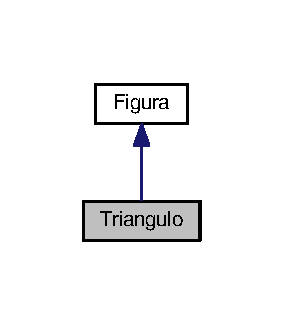
\includegraphics[width=136pt]{classTriangulo__coll__graph}
\end{center}
\end{figure}
\subsection*{Public Member Functions}
\begin{DoxyCompactItemize}
\item 
\hyperlink{classTriangulo_a905d421bd19655a979ccad9e2998db0c}{Triangulo} ()
\item 
\hyperlink{classTriangulo_ab29b2c829712fa6d7ea313373e0d5262}{Triangulo} (double l1, double l2, double l3)
\item 
virtual \hyperlink{classTriangulo_aca2be15b19831e8d7a5331808f5c1958}{$\sim$\+Triangulo} ()
\item 
virtual double \hyperlink{classTriangulo_a1c71a04df8caa1bcb52898636fb20004}{area} ()
\item 
virtual double \hyperlink{classTriangulo_a6f5c542675a726b35f48f953bb2d9acf}{perimetro} ()
\item 
void \hyperlink{classTriangulo_af7fc480161706ec74ece32e9ef1fed7f}{operator$\sim$} ()
\item 
void \hyperlink{classTriangulo_ae0552ffa9641d36e1f571349e5de1070}{operator!} ()
\end{DoxyCompactItemize}
\subsection*{Additional Inherited Members}


\subsection{Detailed Description}
Clase que representa un triángulo. Hereda de la clase figura. 

\subsection{Constructor \& Destructor Documentation}
\index{Triangulo@{Triangulo}!Triangulo@{Triangulo}}
\index{Triangulo@{Triangulo}!Triangulo@{Triangulo}}
\subsubsection[{\texorpdfstring{Triangulo()}{Triangulo()}}]{\setlength{\rightskip}{0pt plus 5cm}Triangulo\+::\+Triangulo (
\begin{DoxyParamCaption}
{}
\end{DoxyParamCaption}
)}\hypertarget{classTriangulo_a905d421bd19655a979ccad9e2998db0c}{}\label{classTriangulo_a905d421bd19655a979ccad9e2998db0c}
Constructor por defecto. Crea un triángulo de lados 3, 4 y 5. \index{Triangulo@{Triangulo}!Triangulo@{Triangulo}}
\index{Triangulo@{Triangulo}!Triangulo@{Triangulo}}
\subsubsection[{\texorpdfstring{Triangulo(double l1, double l2, double l3)}{Triangulo(double l1, double l2, double l3)}}]{\setlength{\rightskip}{0pt plus 5cm}Triangulo\+::\+Triangulo (
\begin{DoxyParamCaption}
\item[{double}]{l1, }
\item[{double}]{l2, }
\item[{double}]{l3}
\end{DoxyParamCaption}
)}\hypertarget{classTriangulo_ab29b2c829712fa6d7ea313373e0d5262}{}\label{classTriangulo_ab29b2c829712fa6d7ea313373e0d5262}
Constructor que recibe la longitud de los tres lados del triángulo. Verifica que los lados tengan una longitud válida, de lo contrario imprime un mensaje de error y construye un triángulo de lados 3, 4 y 5. 
\begin{DoxyParams}{Parameters}
{\em l1} & Uno de los lados. \\
\hline
{\em l2} & Uno de los lados. \\
\hline
{\em l3} & Uno de los lados. \\
\hline
\end{DoxyParams}
\index{Triangulo@{Triangulo}!````~Triangulo@{$\sim$\+Triangulo}}
\index{````~Triangulo@{$\sim$\+Triangulo}!Triangulo@{Triangulo}}
\subsubsection[{\texorpdfstring{$\sim$\+Triangulo()}{~Triangulo()}}]{\setlength{\rightskip}{0pt plus 5cm}Triangulo\+::$\sim$\+Triangulo (
\begin{DoxyParamCaption}
{}
\end{DoxyParamCaption}
)\hspace{0.3cm}{\ttfamily [virtual]}}\hypertarget{classTriangulo_aca2be15b19831e8d7a5331808f5c1958}{}\label{classTriangulo_aca2be15b19831e8d7a5331808f5c1958}
Destructor por defecto. 

\subsection{Member Function Documentation}
\index{Triangulo@{Triangulo}!area@{area}}
\index{area@{area}!Triangulo@{Triangulo}}
\subsubsection[{\texorpdfstring{area()}{area()}}]{\setlength{\rightskip}{0pt plus 5cm}double Triangulo\+::area (
\begin{DoxyParamCaption}
{}
\end{DoxyParamCaption}
)\hspace{0.3cm}{\ttfamily [virtual]}}\hypertarget{classTriangulo_a1c71a04df8caa1bcb52898636fb20004}{}\label{classTriangulo_a1c71a04df8caa1bcb52898636fb20004}
Calcula el área del triángulo. \begin{DoxyReturn}{Returns}
El resultado del cálculo. 
\end{DoxyReturn}


Reimplemented from \hyperlink{classFigura_ade6b12995c86cb72e37738668d77963d}{Figura}.

\index{Triangulo@{Triangulo}!operator"!@{operator"!}}
\index{operator"!@{operator"!}!Triangulo@{Triangulo}}
\subsubsection[{\texorpdfstring{operator"!()}{operator!()}}]{\setlength{\rightskip}{0pt plus 5cm}void Triangulo\+::operator! (
\begin{DoxyParamCaption}
{}
\end{DoxyParamCaption}
)}\hypertarget{classTriangulo_ae0552ffa9641d36e1f571349e5de1070}{}\label{classTriangulo_ae0552ffa9641d36e1f571349e5de1070}
Imprime el area y el perimetro. \index{Triangulo@{Triangulo}!operator````~@{operator$\sim$}}
\index{operator````~@{operator$\sim$}!Triangulo@{Triangulo}}
\subsubsection[{\texorpdfstring{operator$\sim$()}{operator~()}}]{\setlength{\rightskip}{0pt plus 5cm}void Triangulo\+::operator$\sim$ (
\begin{DoxyParamCaption}
{}
\end{DoxyParamCaption}
)}\hypertarget{classTriangulo_af7fc480161706ec74ece32e9ef1fed7f}{}\label{classTriangulo_af7fc480161706ec74ece32e9ef1fed7f}
Imprime los datos del triangulo. \index{Triangulo@{Triangulo}!perimetro@{perimetro}}
\index{perimetro@{perimetro}!Triangulo@{Triangulo}}
\subsubsection[{\texorpdfstring{perimetro()}{perimetro()}}]{\setlength{\rightskip}{0pt plus 5cm}double Triangulo\+::perimetro (
\begin{DoxyParamCaption}
{}
\end{DoxyParamCaption}
)\hspace{0.3cm}{\ttfamily [virtual]}}\hypertarget{classTriangulo_a6f5c542675a726b35f48f953bb2d9acf}{}\label{classTriangulo_a6f5c542675a726b35f48f953bb2d9acf}
Calcula el perímetro del triángulo. \begin{DoxyReturn}{Returns}
El resultado del cálculo. 
\end{DoxyReturn}


Reimplemented from \hyperlink{classFigura_a7451dfc1da3533fa15205df11afe7ac3}{Figura}.



The documentation for this class was generated from the following files\+:\begin{DoxyCompactItemize}
\item 
include/triangulo.\+h\item 
source/triangulo.\+cpp\end{DoxyCompactItemize}

%--- End generated contents ---

% Index
\backmatter
\newpage
\phantomsection
\clearemptydoublepage
\addcontentsline{toc}{chapter}{Index}
\printindex

\end{document}
